\section{Interface}
\subsection{Vue Interface}

\par L'interface utilisé est séparé horizontalement pour les 2 plateaux de jeu, qui sont chacun la grille d'un des joueurs. Le fond est de couleur bleu, tandis que toute la grille et ses coordonnées sont en noir. 
\par Les bateaux sont représenté par des ovales blancs qui recouvrent toutes les cases de ce bateau. Ces dernier ne sont visible que pour la grille du joueur Humain, et des grilles des joueurs non Humain uniquement lorsque ceux ci sont coulé.
\par Les cases touchées par un tir sont recouvert d'un cercle rouge ou vert, indiquant respectivement si un bateau s'y situe ou non.
\begin{figure}[H]
    \centering
    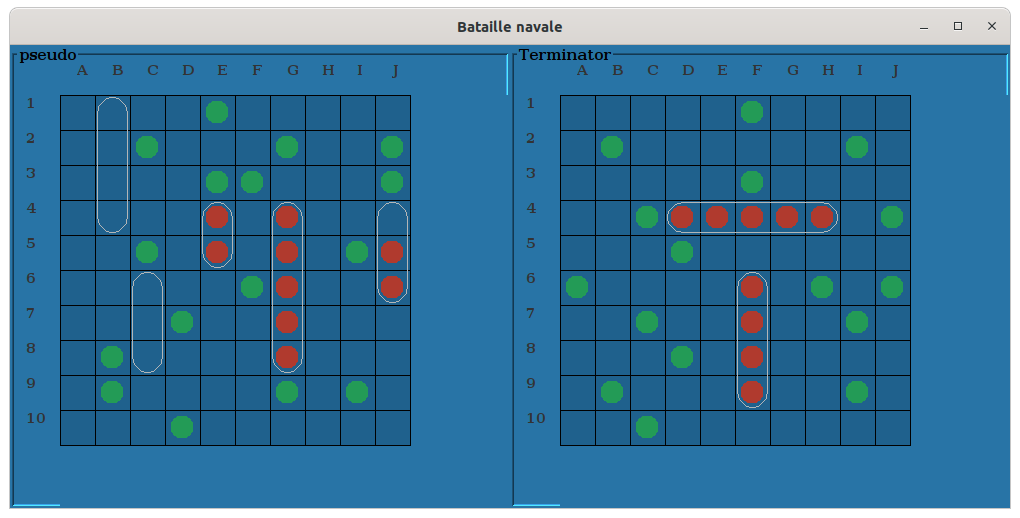
\includegraphics[scale=0.35]{images/interface/PartieEnCours.png}
    \caption{\label{fig: PartieEnCoursI} Interface après quelques coups}
\end{figure}
\par L'interface a une taille fixe de base, mais elle peut être ré redimensionné à sa guise, les grilles s'adaptant à la taille de la fenêtre en permanence. 

\subsection{Contrôleur Interface}
\par Le contrôleur interface quand a lui ouvre plusieurs fenêtres. Les premières fenêtres sont les fenêtres de personnalisation ou l'on demande : \begin{itemize}
    \item Le nom (ou pseudo) de l'utilisateur,
        \begin{figure}[htp]
        \centering
        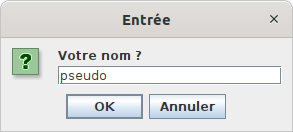
\includegraphics[scale=0.5]{images/interface/ChoixNom.png}
        \caption{\label{fig: ChoixNomI}Fenêtre de personnalisation N°1 : Choix du nom}
        \end{figure}
    \item La version de l'IA adverse (RandomPlayer ou IAPlayer),
        \begin{figure}[htp]
        \centering
        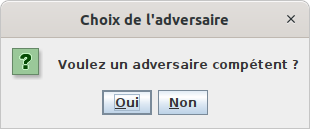
\includegraphics[scale=0.5]{images/interface/ChoixAdversaire.png}
        \caption{\label{fig: ChoixAdversaireI}Fenêtre de personnalisation N°2 : Choix de l'adversaire}
        \end{figure}
    \item Le placement manuel ou aléatoire de nos bateaux .\\
    \begin{figure}[htp]
    \centering
        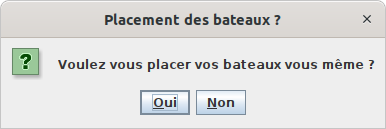
\includegraphics[scale=0.5]{images/interface/ChoixPlacement.png}
        \caption{\label{fig: ChoixPlacementI}Fenêtre de personnalisation N°3 : Choix du Placement}
    \end{figure}
\end{itemize}
    
\par Une fois que toutes les fenêtres de personnalisations sont complétées la fenêtre principale s'ouvre. \\
\par Similairement au Contrôleur terminal, le joueur devra placer ses bateaux un à un, du plus grand au plus petit.
\par Pour cela le joueur devra cliquer sur une case de son plateau, qui sera la coordonnée de départ de celui ci, puis une fenêtre s'ouvrira et demandera l'orientation désirée pour le bateau. \\ Si l'emplacement du bateau est correct, il est placé et on continue avec le prochain, sinon un fenêtre d'erreur indique le problème du placement du bateau. \\ En cas d'erreur lors du clic initial, il est possible d'annuler la création du bateau, mais une fois celui ci placé il ne peut plus être enlevé.
\par Une fois le placement effectué, la partie commence .
\par Dans une partie humain contre ordinateur, le joueur Humain joue en premier en cliquant sur une case du plateau adverse. Cette action fera un coup sur la case et appliquera ce coup sur le modèle puis mets la vue a jour.
\par L'ordinateur répliquera, et ainsi de suite, jusqu'à qu'un joueur ait coulé tout les bateaux de l'autre, ce qui résulte en une fenêtre qui félicite le gagnant, puis fermera le jeu.